\chapter{Implementación}
\label{ch:implementacion}

\section{Estructura}
\label{ch:implementacion:sec:estructura}

Para realizar la implementacion del algoritmo se debe primero proponer una convención para enumerar los vertices y aristas de un cubo, para esta implementacion se usará la convención señalada anteriormente en la figura \ref{f:estadoDelArte:convention}, luego de definida la enumeración de cada vértice y arista, es necesario poder representar cada uno de los 256 casos con un identificador único denominado \emph{cubeIndex}, luego hay que determinar que aristas son cortadas por la superficie que atraviesa cada caso en particular, para ello se necesita de una tabla que asocie un \emph{cubeIndex} con las aristas que serán atravesadas, esta tabla se denomina \emph{edgeTable}, una vez que se conocen aquellas aristas que son atravesadas, el siguiente paso es crear una malla de triángulos que formen esta superficie, la tabla \emph{triTable} asocia cada caso con una lista de triángulos ordenados, que generan la superficie buscada. Todas estas estructuras de datos serán explicadas a continuación.

\section{Estructuras de datos}
\label{ch:implementacion:sec:estructurasDeDatos}

\subsection{CubeIndex}
\label{ch:implementacion:sec:CubeIndex}

Como se mencionó en \ref{subsec:marchingCubes:consideracionesGeometricas}, existen 256 formas posibles de atravesar un cubo con una superficie continua, que es lo mismo decir, existen 256 combinaciones posibles dados 8 vertices que pueden estar en 2 estados distintos (indicando que están dentro de una superficie cerrada o fuera de ésta)

Para poder identificar cada uno de estos 256 casos, se enumeran del 1 al 256 usando un arreglo de 8 bits, basándose en el estado de cada vértice usando la convención, por ejemplo, un cubo que tiene todos sus vértices marcados como fuera de la superficie (externos), tiene todos sus bits en cero, por lo tanto, el índice, desde ahora \emph{cubeIndex}, de este cubo es \hbox{$0_{10} = 0000 \; 0000_{2}$} (cero), de la misma manera, usando la convención, si un cubo sólo tiene el tercer vertice (vertice 2), dentro de la superficie, entonces, tiene su tercer bit en 1, y el resto en cero, luego el \emph{cubeIndex} del cubo es $4_{10} = 0000 \; 0100_{2}$, si un cubo es atravesado por la mitad, dejando a la mitad de abajo dentro de la superficie, tiene los vértices 4, 5, 6 y 7 marcados como internos, por lo que los bits 4, 5, 6 y 7 (los ultimos 4), valen 1, por lo tanto, el \emph{cubeIndex} es $240_{10} = 1111 \; 0000_{2}$.

En general, el \emph{cubeIndex} se determina como se muestra en la figura \ref{f:ch:implementacion:sec:CubeIndex:cubeindex:cubeindex}.

\begin{figure}[hbt]
	\makebox[\textwidth]{\framebox[0.9\textwidth]{\rule{0pt}{0.3\textwidth}}}
	\caption{Como se usan los vértices como bits ordenados para formar el \emph{cubeIndex}}
	\label{f:ch:implementacion:sec:CubeIndex:cubeindex:cubeindex}
\end{figure}

\subsection{edgeTable}
\label{ch:implementacion:sec:edgeTable}

Luego de establecer como identificar un cubo, es necesario poder conocer que aristas serian intersectadas por la superficie, para poder determinar un punto sobre estas aristas por las cuales se sostendrá un triángulo. Por ejemplo, si el vértice $0$, es el unico vértice que queda dentro de la superficie, usando la convención, se puede asumir las aristas $0$, $3$ y $8$ serán aquellas las cuales la superficie intersectara a cubo.

Es por esto que se necesita una forma de relacionar un \emph{cubeIndex} con las aristas que serán atravesadas por la superficie.

Usando la misma estrategia que con el \emph{cubeindex} existen 4096 $(2^{12})$ combinaciones posibles de tomar 12 aristas que pueden intersectar a la superficie o no, por esto, cada caso, será identificado con un numero de 12 bits, en el cual, cada bit representa a una arista, usando la convención como se muestra en la figura \ref{f:ch:implementacion:sec:CubeIndex:edgeTable:edge_convention}.

\begin{figure}[hbt]
	\makebox[\textwidth]{\framebox[0.4\textwidth]{\rule{0pt}{0.3\textwidth}}}
	\caption{Convención para enumerar las 4096 combinaciones posibles de aristas}
	\label{f:ch:implementacion:sec:CubeIndex:edgeTable:edge_convention}
\end{figure}

La \emph{edgeTable} es un \emph{array} (arreglo) diseñado para asociar un \emph{cubeindex} con quellas aristas que son intersectadas. Este \emph{array} consta de 256 numeros (uno por cada caso o cada \emph{cubeindex}) de 12 bits, un bit para cada una de las 12 aristas del cubo en cuestión por las cuales pasa la superficie.

Para entender mejor, se supone el ejemplo de la figura \ref{f:ch:implementacion:sec:CubeIndex:edgeTable:example}.

\begin{figure}[hbt]
	\makebox[\textwidth]{\framebox[0.3\textwidth]{\rule{0pt}{0.2\textwidth}}}
	\caption{Un cubo cuyo vértice $0$ es el único marcado.}
	\label{f:ch:implementacion:sec:CubeIndex:edgeTable:example}
\end{figure}

En este ejemplo, sólamente el vértice $0$, ha sido marcado como interno, luego, el \emph{cubeIndex} es $1_{10} = 0000 \; 0001_{2}$, dado esto, las aristas $0$, $3$ y $8$ serán eventualmente atravesadas por la superficie, por lo tanto:

\begin{quote}
	edgeTable[1] = 0x109
\end{quote}

Lo cual tiene un valor equivalente a: $109_{16} = 265_{10} = 0001 \; 0000 \; 1001_{2}$, lo que indica, viendo la notacion binaria, que las aristas $0$, $3$ y $8$ son las que serán atravesadas.

Otro ejemplo, se supone el caso de la figura \ref{f:ch:implementacion:sec:CubeIndex:edgeTable:example}

\begin{figure}[hbt]
	\makebox[\textwidth]{\framebox[0.3\textwidth]{\rule{0pt}{0.2\textwidth}}}
	\caption{Un cubo cuyos vértices $5$ y $6$ son los únicos marcados.}
	\label{f:ch:implementacion:sec:CubeIndex:edgeTable:example}
\end{figure}

En este caso, los vértices $5$ y $6$ han sido marcados como internos, luego, el \emph{cubeIndex} debe ser: $96_{10} = 0110 \; 0000_{2}$, por lo tanto la superficie deberia atravesar las aristas $4$, $9$, $6$ y $10$, para que asi, una superficie deje a estos vértices separados del resto.

Para saber que aristas finalmente son atravesadas, se debe consultar a la tabla \emph{edgeTable}, usando como índice, el \emph{cubeIndex} calculado anteriormente.

\begin{quote}
	edgeTable[96] = 0x650
\end{quote}

El valor entregado por la \emph{edgeTable} para el \emph{cubeIndex} $96$, es $0x650$ (hexadecimal), lo que es equivalente a:

\begin{quote}
	$650_{16} = 1616_{10} = 0110 \; 0101 \; 0000_{2}$
\end{quote}

Según la notación binaria, se puede ver que el valor entregado por la tabla \emph{edgeTable}, indica que los vertices $4$, $6$, $9$ y $10$ son aquellos que son atravesados por la superficie, de forma que los vertices $5$ y $6$ queden separados del resto.

\subsection{triTable}
\label{ch:implementacion:sec:triTable}

Una vez que se conocen aquellas aristas que seran atravesadas, es momento de crear la superficie interna que atraviese estas aristas y separe los vertices marcados de los demás. Para ello, es necesario poder generar aquellos triángulos que formen esta superficie.

la tabla \emph{triTable} es una tabla de 256 \emph{arrays} (arreglos) de 16 numeros cada uno, hay un arreglo por cada uno de los 256 casos descritos en \ref{ch:implementacion:sec:CubeIndex}, en cada caso, es necesario generar una serie de triángulos que describirán la superficie, y de todos los casos, como máximo se necesitan 5 triángulos para los casos mas complejos.

Analizando un caso simple, un cubo que solamente tiene un vértice marcado, por lo tanto se necesita tan sólo un triángulo que se sostenga de las aristas que convergen en ese vertice, para asi crear una superficie que atraviese el cubo dejando a ese vértice separado del resto de los vértices del cubo, es por esto, que el segundo elemento (\emph{cubeIndex} = 1) de la tabla \emph{triTable} tiene un valor:

\begin{quote}
	$triTable[1] = \{0, 8, 3, -1, -1, -1, -1, -1, -1, -1, -1, -1, -1, -1, -1, -1\}$
\end{quote}

Esto indica que el primer triángulo, es aquel que se sostiene (o corta) de las aristas: $0$, $8$ y $3$.

El resto de los $13$ números que quedan tienen un valor de $-1$, lo cual permite a cualquier implementacion del algoritmo, iterar en los numeros como tripletas, y detenerse cuando el primer número tenga un valor de $-1$.

De esta manera, cuando un cubo no tiene ninguno de sus vértices marcados (\emph{cubeIndex} = 0), o tiene todos sus vértices marcados (\emph{cubeIndex} = 255), los valores de la triTable para ambos casos son:

\begin{quote}
	$triTable[0]	= \{-1, -1, -1, -1, -1, -1, -1, -1, -1, -1, -1, -1, -1, -1, -1, -1\}$\\
	$triTable[255]	= \{-1, -1, -1, -1, -1, -1, -1, -1, -1, -1, -1, -1, -1, -1, -1, -1\}$
\end{quote}

Esto indica que para ambos casos, no se crea ningún trianglo, ya que cuando no tiene ningún vértice marcado indica que esta completamente fuera de la superficie, o en el otro caso, el cubo está contenido completamente dentro de la superficie, y ambos casos deben ser reemplazados por un cubo con cero triangulos.

\section{Datos de entrada}
\label{ch:implementacion:sec:datosDeEntrada}

\subsection{Requerimientos}
\label{ch:implementacion:sec:datosDeEntrada:subsec:requerimientos}

Para poder utilizar el algoritmo de \emph{MarchingCubes}, se necesita que cada punto de un espacio tridimensional tenga asociado un valor dentro de un rango definido de manera que cada punto pueda describirse como un vector de cuatro dimensiones compuestas por sus coordenadas y un valor escalar, como muestra la ecuacion \ref{ch:implementacion:sec:datosDeEntrada:vector}.

\begin{equation}
\label{ch:implementacion:sec:datosDeEntrada:vector}
	(x,y,z,v)
\end{equation}

Por ejemplo, en una habitación se tiene un foco de luz en el centro emitiendo luz en todas direcciones, con esto, cada punto de la habitación percibe distintas instensidades de luz que depende de la distancia al foco, mientras mas cerca del foco, mayor intensidad, mientras mas alejado del foco, menor intensidad. Si de alguna manera pudiesen marcase todos aquellos puntos que tengan una intensidad especifica se tendria una esfera formada por puntos equidistantes al foco, ya que todo ellos comparten la misma intensidad, por lo que se dice que esa es la superficie que encierra a todos los puntos con una cierta intensidad o mayor.

Ciertamente, el algoritmo tambien sirve para visualizar graficos en tres dimensiones, usando el mismo principio, cada punto del espacio tiene un valor asociado el cual es calculado por la ecuacion, para poder dibujar la susperficie se puede transformar la ecuacion en una inecuacion y luego marcar todos aquellos puntos que sean menores que el valor entregado por la ecuacion, por ejemplo se tiene en la ecuación \ref{ch:implementacion:sec:datosDeEntrada:ec1}:

\begin{equation}
\label{ch:implementacion:sec:datosDeEntrada:ec1}
	x^{2} + y^{2} = 1
\end{equation}

Para poder graficar esta ecuacion usando \emph{MarchingCubes} se debe transformar la ecuación en una inecuación como se muestra en la ecuacion \ref{ch:implementacion:sec:datosDeEntrada:ec2}:

\begin{equation}
\label{ch:implementacion:sec:datosDeEntrada:ec2}
	x^{2} + y^{2} <= 1
\end{equation}

Dependiendo de la resolución escogida, es posible que algunos cubos tengan algunos de sus vértices con coordenadas $(x,y)$ que satisfacen a la inecuación, por lo tanto quedan marcados como vértices internos, luego el proceso es ir iterando en todos esos cubos y reemplazando los cubos por los triangulos que correspondan a los quince casos mostrados en la figura \ref{f:estadoDelArte:MarchingCubes}.

\subsection{Datos como cortes de nivel}
\label{ch:implementacion:sec:datosDeEntrada:subsec:datoscomocurvasdenivel}

Otra forma de entregar datos de entrada es teniendo cortes de nivel de un cuerpo tridimensional, un ejemplo de esto son las imágenes obtenidas de los exámenes de resonancia magnética. Cada imagen representa un corte transversal del cuerpo estudiado, como el que se muestra en la figura \ref{f:ch:implementacion:sec:datosdeentrada:img:ejemplodernm}:

\begin{figure}[hbt]
	\makebox[\textwidth]{\framebox[0.5\textwidth]{\rule{0pt}{0.5\textwidth}}}
	\caption{Imágenes una resonancia magnética de abdomen completo}
	\label{f:ch:implementacion:sec:datosdeentrada:img:ejemplodernm}
\end{figure}

Éstas imágenes, en conjunto, describen un cuerpo en tres dimensiones, mostrando con detalle sus componentes internos. Cada imágen está compuesta por una matriz de pixeles en una escala de grises, dependiendo de la profundidad de color, pueden ser de 256 valores (8 bits) o de 65536 valores (16 bits) diferentes, con estas imágenes se puede construir un espacio que puede servir como entrada para el algoritmo de \emph{MarchingCubes}, una un de hacerlo es usando las coordenadas en 2 dimensiones del pixel en una imagen y usando como valor $z$, el número que representa la imagen dentro del cuerpo, una vez identificado el pixel en un espacio tridimensional, el valor de éste pixel está determinado por la intensidad de color del pixel, como se muestra en la ecuación \ref{ch:implementacion:sec:datosDeEntrada:ec3}:

\begin{equation}
\label{ch:implementacion:sec:datosDeEntrada:ec3}
	(x,y,z,color)
\end{equation}

Para ejemplificar, considere dos imágenes de $2x2$ pixeles, esto crea 8 pixeles en total, suficientes para que cada pixel represente un vértice de un cubo, luego cada pixel determina el valor del vértice usando la tonalidad gris del pixel asociado. En la figura \ref{f:implementacion:images_minimal}, se muestra éste caso, usando 2 imágenes cuyos pixeles tienen una tonalidad de gris de 97, en una escala de 0 a 255 (8 bits), excepto el pixel (0,0) de la primera imagen (imagen \#0).

\begin{figure}[!hbt]
	\centering
	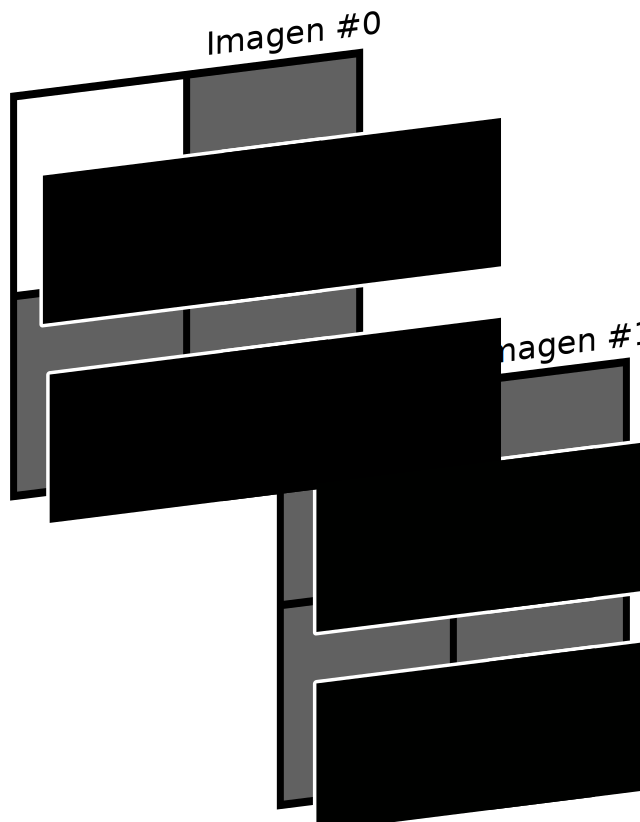
\includegraphics[width=0.6\textwidth]{images/misc/images_minimal.pdf}
	\caption{Dos imágenes de $2x2$ pixeles cada una, cada pixel está etiquetado con su respectivo vector de 4 dimensiones.}
	\label{f:implementacion:images_minimal}
\end{figure}

Si se aplica \emph{Marching Cubes} en este caso usando un valor mínimo de $100$, casi todos los vértices cumplirian la condición ya que casi todos los vértices tienen un valor de $97$, excepto el vértice correspondiente al pixel $(0,0,0)$ (primer pixel de la imagen \#0), por esto, es el único vértice no marcado, quedando asi un cubo que solo necesita de un sólo triángulo que separa a este vértice de los demás, como se muestra en la figura \ref{f:implementacion:images_minimal_cube}.

\begin{figure}[!hbt]
	\centering
	
\includegraphics[width=0.3\textwidth]{images/misc/images_minimal_cube.pdf}
	\caption{El resultado de aplicar \emph{Marching Cubes}, solo se obtiene un triángulo que separa al vertice blanco, de los demás.}
	\label{f:implementacion:images_minimal_cube}
\end{figure}

\pagebreak
En esta implementación, se usó este último método para obtener una nube de puntos para poder extraer una superficie utilizando \emph{Marching Cubes}.

%TODO: poner link al glosario, en 'dataset'
Las imágenes de la figura \ref{f:implementacion:dataset:ImSphRad100} muestran algunas de las imágenes de un \emph{dataset} que describe una esfera mediante cortes transversales.

\begin{figure}
\centering

	\begin{subfigure}{0.30\textwidth}
		\centering
		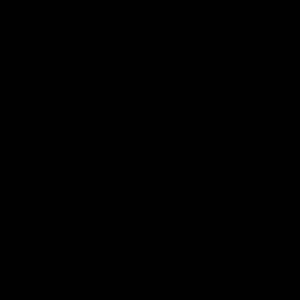
\includegraphics[width=\textwidth]{images/datasets/ImSphRad100/Sphere001.png}
		\caption{Imagen \#001}
		\label{f:implementacion:ImSphRad100:001}
	\end{subfigure}
	%~
	\begin{subfigure}{0.30\textwidth}
		\centering
		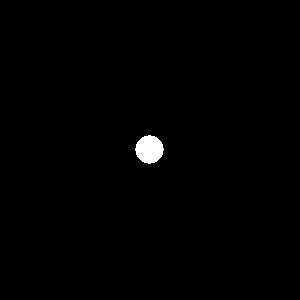
\includegraphics[width=\textwidth]{images/datasets/ImSphRad100/Sphere051.png}
		\caption{Imagen \#051}
		\label{f:implementacion:ImSphRad100:051}
	\end{subfigure}
	%~
	\begin{subfigure}{0.30\textwidth}
		\centering
		
\includegraphics[width=\textwidth]{images/datasets/ImSphRad100/Sphere070.png}
		\caption{Imagen \#070}
		\label{f:implementacion:ImSphRad100:070}
	\end{subfigure}

	\begin{subfigure}{0.30\textwidth}
		\centering
		
\includegraphics[width=\textwidth]{images/datasets/ImSphRad100/Sphere102.png}
		\caption{Imagen \#102}
		\label{f:implementacion:ImSphRad100:102}
	\end{subfigure}
	%~
	\begin{subfigure}{0.30\textwidth}
		\centering
		
\includegraphics[width=\textwidth]{images/datasets/ImSphRad100/Sphere166.png}
		\caption{Imagen \#166}
		\label{f:implementacion:ImSphRad100:166}
	\end{subfigure}
	%~
	\begin{subfigure}{0.30\textwidth}
		\centering
		
\includegraphics[width=\textwidth]{images/datasets/ImSphRad100/Sphere218.png}
		\caption{Imagen \#218}
		\label{f:implementacion:ImSphRad100:218}
	\end{subfigure}

	\begin{subfigure}{0.30\textwidth}
		\centering
		
\includegraphics[width=\textwidth]{images/datasets/ImSphRad100/Sphere241.png}
		\caption{Imagen \#241}
		\label{f:implementacion:ImSphRad100:241}
	\end{subfigure}
	%~
	\begin{subfigure}{0.30\textwidth}
		\centering
		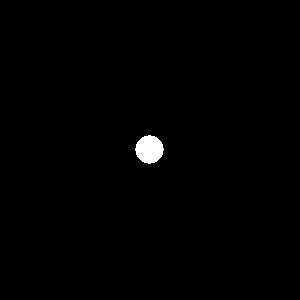
\includegraphics[width=\textwidth]{images/datasets/ImSphRad100/Sphere249.png}
		\caption{Imagen \#249}
		\label{f:implementacion:ImSphRad100:249}
	\end{subfigure}
	%~
	\begin{subfigure}{0.30\textwidth}
		\centering
		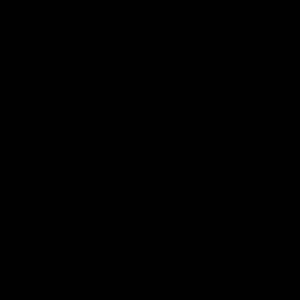
\includegraphics[width=\textwidth]{images/datasets/ImSphRad100/Sphere300.png}
		\caption{Imagen \#300}
		\label{f:implementacion:ImSphRad100:300}
	\end{subfigure}

	\caption{Imágenes que describen una esfera}
	\label{f:implementacion:dataset:ImSphRad100}
\end{figure}

Éste dataset consta de 300 imágenes de $300 x 300$ pixeles con una profundidad de grises de 8 bits. Como se puede observar en la imagen \ref{f:implementacion:ImSphRad100:001} todos sus pixeles son negros, y considerando una profundidad de grises de 8 bits, es que todos sus pixeles valen $0$ (cero), sin embargo, la imagen \label{f:implementacion:ImSphRad100:051} muestra un pequeño círculo en su centro, por lo que aquellos pixeles que estan dentro del círculo, tienen un valor de $FF_{16} = 00_{2}$. A medida que nos acercamos a la imagen numero 300, este cŕculo va creciendo hasta alcanzar un radio máximo, luego, su radio comienza a disminuir, hasta volver a un valor de cero. Describiendo de esta manera una esfera, en un espacio discreto de puntos de tamaño $300 x 300 x 300$

Ya que cada pixel, tiene asociado un par de coordenadas en 2 dimensiones, un número de imágen, y además un valor para especificar una tonalidad de gris, se puede describir cada pixel, como un vector de 4 dimensiones como se explicó en la seccion \ref{ch:implementacion:sec:datosDeEntrada:subsec:requerimientos}. Satisfaciendo los requerimientos que necesitan los datos de entrada para poder usar \emph{Marching Cubes}.

El resultado de aplicar \emph{Marching Cubes} a este \emph{dataset} se muestra en la figura \ref{f:implementacion:ImSphRad100:screenshot_40}, se puede apreciar como la esfera está formada por cortes transversales, cada uno describe un circulo cuyo radio va en aumento, y a medida que se acerca al final, disminuye. Además, se puede ver el efecto de escalonamiento (\emph{aliasing}) que presenta la superficie debido al uso de \emph{Marching Cubes}.

\begin{figure}[hbt]
	\centering
	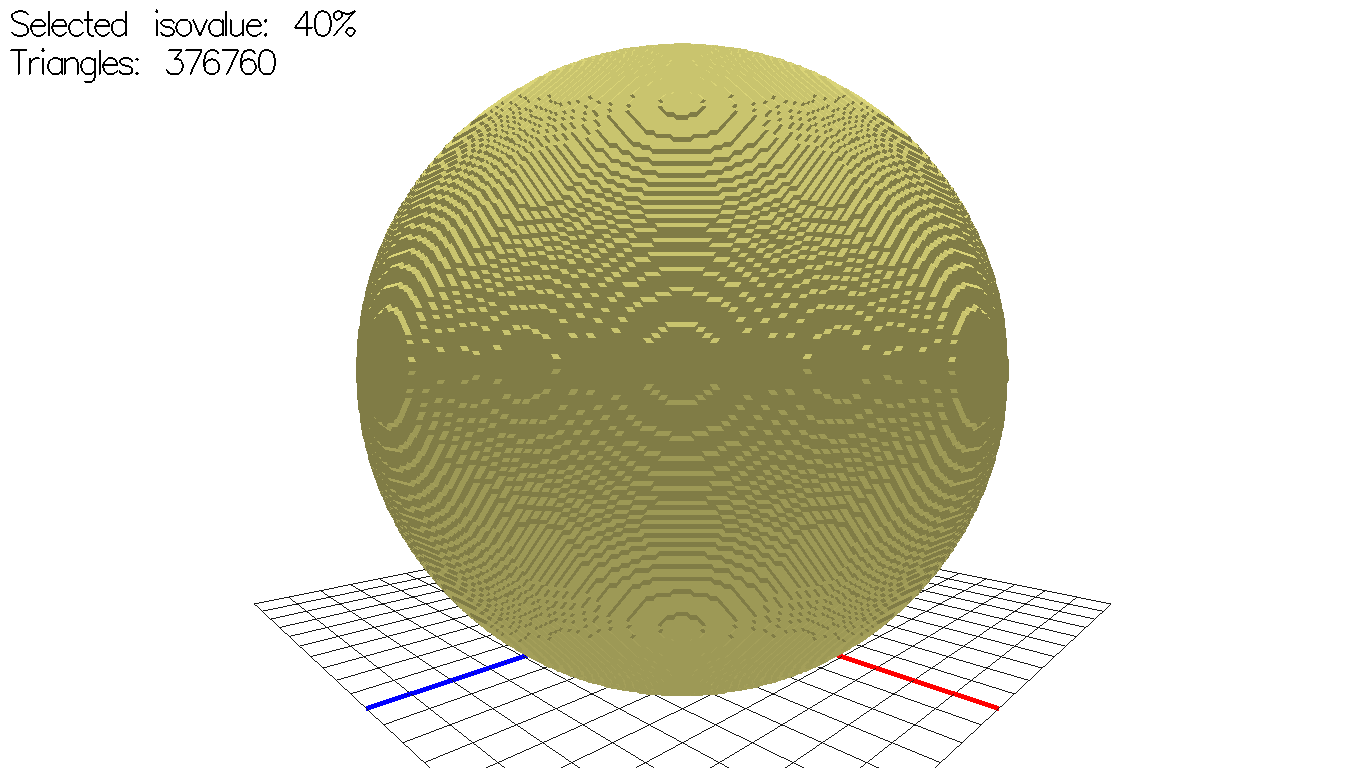
\includegraphics[width=0.95\textwidth]
	{images/results/ImSphRad100/screenshot_40.png}
	\caption{La superficie extraida usando \emph{Marching Cubes} sobre un dataset que describe una esfera.}
	\label{f:implementacion:ImSphRad100:screenshot_40}
\end{figure}

\subsection{Formato de las imágenes de entrada}
\label{ch:implementacion:sec:datosDeEntrada:subsec:formatodelasimagenesdeentrada}

Idealmente, las imágenes utilizadas deberian estar todas en el mismo formato y compresión para ser utilizadas, también con la misma profundidad de colores (8 o 16 bits), pero esto no siempre es asi.

%TODO: poner referencias a los formatos de imagenes, como svg y eso
Debido a que las imágenes provienen de orígenes y propósitos distintos, son obtenidas por distintos métodos, por ejemplo, uno puede crear imágenes de curvas de nivel de una ecuacion tridimensional y un \emph{dataset} de imágenes en algún formato vectorial como SVG. En el campo de la imagenología se usa el formato DICOM para la distribucion digital de imágenes médicas, en las cuales, dentro de las imágenes hay información del paciente y otros datos relacionados con el estudio. De la misma manera, para efectos de investigación y publicación, se pueden encontrar en internet algunos \emph{datasets} que vienen en formato RAW, es decir, sin compresion alguna, y sin informacion alguna, solo un arreglo de bytes los cuales representan un pixel de 8 bits continuados, para poder leer estos archivos es necesario conocer anticipadamente las dimensiones tridimensionales del \emph{dataset}.

El algoritmo de \emph{Marching Cubes} es indiferente de cómo se obtengan los datos de entrada, mientras éstos puedan ser expresados como una nube de puntos tridimensionales, cada uno con un valor asociado dentro de un rango definido, como se explicó en la seccion \ref{ch:implementacion:sec:datosDeEntrada:subsec:requerimientos}, por lo que para usar un \emph{dataset} de imágenes, la implementacion debe poder extraer esta nube de puntos y valores asociados de manera transparente.

Para lograr esta transparencia, se utilizará un único formato de imagen, de manera que el programa pueda extraer los datos sin tener que preocuparse por distinguir entre distintos formatos.

Esto conlleva a que para poder leer un \emph{dataset} de imágenes, sean necesarios dos pasos:

\begin{enumerate}
	\item Convertir las imágenes del \emph{dataset} al formato único admitido.
	\item Procesar las imágenes convertidas y extraer los puntos y sus valores
\end{enumerate}

Este esquema permite que cualquier \emph{dataset} de imágenes pueda ser utilizado, sin importar el formato de origen, logrando que el formato de entrada dea completamente transparente para el algoritmo que finalmente tomará las nubes de puntos como entrada.

\section{Formato único escogido}
\label{ch:implementacion:sec:formatounicoescogido}

%TODO: citas
% http://netpbm.sourceforge.net/history.html
El formato de imagen escogido es el formato PGM (\emph{Portable GreyMap}), el cual derivado del formato PBM (\emph{Portable BitMap}) inventado por Jef Poskanzer en los años 1980, cuyo proposito era crear un formato libre de problemas, resistente a los cambios de codificación a través de correo electrónico, para mapas de bits (\emph{bitmaps}) en blanco y negro. Fue diseñado para ser lo suficientemente simple para que una imagen pudiese ser transmitida por correo electrónico sin nigún método de encapsulamiento especial y sobrevivir a cualquier traducción y ser facilmente extraible en el correo destino.

\subsection{Historia}
\label{ch:implementacion:sec:formatounicoescogido:subsec:historia}

En el año 1988, Jef distribuyó herramientas para trabajar con las imágenes PBM, en un proyecto conocido como \emph{Pbmplus}, éstas fueron las herramientas principales para convertir entre imágenes PBM y otras existentes.

A finales de 1988, Jef agregó los formatos PGM y PPM y muchas mas herramientas al proyecto \emph{Pbmplus}, finalmente, aunque Jef jamás renunció de manera formal a dar soporte al proyecto, el 10 de diciembre de 1991 fue su última actualización, y el proyecto quedo abandonado.

En el año 1993, el proyecto \emph{Netbpm} fue desarrollado para reemplazar a \emph{Pbmplus}, este nuevo proyecto no era nada más que un cambio de nombre, llamado así por el hecho de que la gente al rededor del mundo pudiera mantener este paquete hasta el dia de hoy.

\subsection{Formato PGM}
\label{ch:implementacion:sec:formatounicoescogido:subsec:formatopgm}

La especificación de los archivos PGM es simple:

\begin{enumerate}
	\item Un \jcq{número mágico} para identificar el tipo de archivo. En numero mágico de un archivo PGM son dos caracteres: \jcq{P2}, para pixeles escritos como caracteres ASCII, o \jcq{P5}, si los pixeles estan escritos de manera binaria usando 1 o 2 \emph{bytes}
	\item Un caracter de espacio.
	\item Un valor ANCHO, formateado como un caracter ASCII en decimal.
	\item Un caracter de espacio.
	\item Una valor ALTURA, nuevamente como un caracter ASCII en decimal.
	\item Un caracter de espacio.
	\item El valor MÁXIMO para la escala de grises (que representara el color blanco), nuevamente en ASCII decimal, debe ser menor que 65536 (para no superar una profundidad de color de 16 bits), y mayor que cero.
	\item Un caracter de espacio (usualmente una nueva línea).
	\item Una trama de ALTURA filas, ordenadas de arriba hacia abajo, cada fila consiste en una cantidad definida por el valor ANCHO de valores grises, de izquierda a derecha, cada valor de gris es un número entre cero y el definido como MÁXIMO, siendo $0$ el valor que representa al negro, y MÁXIMO el que representa el color blanco, cada valor es representado como un valor binario puro de 1 o 2 bytes, si el valor MÁXIMO es menor a 255, entonces es 1 \emph{byte}, de lo contrario, son 2 bytes. El byte más significativo es el primero.
	Una fila de una imagen es horizontal, y una columna vertical, los pixeles son cuadrados y son contiguos.
\end{enumerate}

Dependiendo del \jcq{Numero Mágico} (\emph{Magic Number}), existen 6 formatos de archivos diferentes, cada formato difiere solamente en la escala de colores que es capaz de representar, como indica la tabla \ref{ch:implementacion:tabla:tiposdearchivospbm}.

\begin{table}[h]
	\centering
	\begin{tabular}{|l|l|l|}
		\hline
		Magic Number	&	Type				&	Encoding\\ \hline
		P1				&	Portable bitmap		&	ASCII \\ \hline
		P2				&	Portable graymap	&	ASCII \\ \hline
		P3				&	Portable pixmap		&	ASCII \\ \hline
		P4				&	Portable bitmap		&	Binary \\ \hline
		P5				&	Portable graymap	&	Binary \\ \hline
		P6				&	Portable pixmap		&	Binary \\ \hline
	\end{tabular}
	\caption{Tipos de imágenes PBM}
	\label{ch:implementacion:tabla:tiposdearchivospbm}
\end{table}

Un ejemplo de una imagen PGM con codificacion ASCII (con un \emph{Magic Number} \jcq{P2}), se presenta en el siguiente archivo PGM:

\begin{verbatim}
P2
#Este ejemplo muestra la palabra "JOE"
18 7
15
0  0  0  0  0  0  0  0  0  0  0  0  0  0  0  0  0  0
0  3  3  3  3  0  0  7  7  7  7  0  0 11 11 11 11  0
0  0  0  3  0  0  0  7  0  0  7  0  0 11  0  0  0  0
0  0  0  3  0  0  0  7  0  0  7  0  0 11 11 11  0  0
0  3  0  3  0  0  0  7  0  0  7  0  0 11  0  0  0  0
0  3  3  3  0  0  0  7  7  7  7  0  0 11 11 11 11  0
0  0  0  0  0  0  0  0  0  0  0  0  0  0  0  0  0  0
\end{verbatim}

La imagen obtenida de este archivo PGM se muestra en la figura \ref{f:implementacion:sec:formatos:pgm_example_1}

\begin{figure}[hbt]
	\centering
	\includegraphics[width=0.95\textwidth]
	{images/misc/pgm_example_1.png}
	\caption{Imagen PGM obtenida usando el codigo del ejemplo (Imagen ampliada, tamaño original es de $18x7$ pixeles)}
	\label{f:implementacion:sec:formatos:pgm_example_1}
\end{figure}

Para efectos de este estudio, se usarán imágenes en escala de grises, por lo que se usarán los archivos PGM con codificación binaria para una lectura mas simple, es decir, con un \jcq{Número Mágico} de \jcq{P5}

\section{Conversion de imágenes de entrada}
\label{ch:implementacion:sec:conversiondeimagenesdeentrada}

Como se indicó en la sección \ref{ch:implementacion:sec:datosDeEntrada:subsec:formatodelasimagenesdeentrada}, el primer paso para extraer una nube de puntos tridimensionales de cualquier \emph{dataset}, es necesario convertir todas las imágenes de éste.

%TODO: cita a http://www.imagemagick.org/
Este proceso no es trivial, ya que existen muchos formatos disponibles y muchas especificaciones distintas, por lo que dar soporte a todas es algo que escapa del objetivo de esta investigación, es por ello que se utilizó una herramienta de codigo abierto (\emph{opensource}) llamada \emph{ImageMagick}

Esta herramienta hace que el primer paso sea muy simple, y generalizado para cualquier tipo de archivo del cual se pueda extraer informacion de sus metadatos (tamaño, profundidad de color, etc), si no fuere éste el caso, por ejemplo, imagenes RAW sin informacion de metadatos, es necesario una agregar información extra en tiempo de ejecución.

La sintáxis del comando a usar es la siguiente:

\begin{verbatim}
convert <archivo origen> <archivo destino>
\end{verbatim}

ImageMagick se hace cargo de intentar comprender en que formato está el archivo de origen, y mediante la extensión escrita en el archivo destino, De esta manera, para convertir una imagen PNG a JPG se puede hacer:

\begin{verbatim}
convert imagen.png imagen.jpg
\end{verbatim}

Usando esta estrategia, es posible obtener una imagen PGM tan solo haciendo el siguiente comando:

\begin{verbatim}
convert imagen.png imagen.pgm
\end{verbatim}

Esto crea una imagen PGM del tipo \jcq{P2}, es decir los pixeles estan escritos dentro del archivo como caracteres ASCII, para generar una imagen PGM del tipo \jcq{P5}, es decir con sus pixeles representados como bytes binarios, es necesario agregar un argumento extra:

\begin{verbatim}
convert imagen.png -compress none imagen.pgm
\end{verbatim}

De esta manera se obtienen imágenes PGM binarias.

\subsection{Ejemplos de conversión}
\label{ch:implementacion:sec:ejemplosdeconversion}

Para poder convertir un dataset completo, existen varios caminos, el usado en esta implementación fue usar un \emph{bash script}.

El codigo fuente es simple, y pretende facilitar el ingreso de datos y otras opciones al comando \emph{convert}:

\begin{verbatim}
#!/bin/bash

usage()
{
cat << EOF

Uso: $0 <options>

Este script transforma todas las imagenes de una cierta carpeta al formato
PGM, y las guarda en un subdirectorio llamado pgm/ dentro de la carpeta
mencionada.

OPCIONES:
	-h	Imprime este mensaje de ayuda de uso
	-d	Carpeta donde estan las imagenes a transformar
	-t	Carpeta destino de imagenes transformadas (default: pgm)
	-r	Argumento -resize usado por ImageMagick (default: 100%)
	-a	Modo sin compresion ASCII de imagemagick (-compress none)
EOF
}

#if [ $# -eq 0 ]; then
#	usage
#	exit
#fi

while getopts "hd:e:t:r:a" opt; do
	case $opt in
		h)
			usage
			;;
		d)
			BASE_DIR=$OPTARG
			;;
		t)
			TARGET_DIR=$OPTARG
			;;
		r)
			RESIZE=$OPTARG
			;;
		a)
			COMPRESS="-compress none"
			;;
	esac
done

#VALORES POR DEFECTO
if [ -z "$BASE_DIR" ]; then BASE_DIR="."; fi
if [ -z "$RESIZE" ]; then RESIZE="100%"; fi
if [ -z "$TARGET_DIR" ]; then TARGET_DIR="pgm"; fi

###########
#EXECUTION#
###########

ARGUMENTS="-verbose -resize $RESIZE $COMPRESS"

#Go to base dir
cd "$BASE_DIR"

#make target dir
if [ ! -d "$TARGET_DIR" ]; then
	mkdir "$TARGET_DIR"
fi 

for f in *; do
	convert "$f" $ARGUMENTS "$TARGET_DIR/$f.pgm"
done
\end{verbatim}

Este \emph{bash script} permite especificar un directorio donde estan las imágenes del dataset, para poder convertirlas, incluso acepta un parámetro \emph{-r} que escala las imágenes porcentualmente o de manera fija, por ejemplo:

\begin{verbatim}
./convert -d directorio_dataset/ -r 50%
\end{verbatim}

El cual toma todas las imágenes dentro del directorio \emph{directorio\_dataset\slash} y las transforma a PGM, luego de reducir su tamaño en un 50\% a